\chapter{Background}

This chapter aims to provide a brief overview of the available tools related to outbound translation, namely Alignment, Machine translation, Quality estimation and Source complexity.

\section{Alignment}

The alignment of parts of texts in parallel corpora is a common task in NLP and especially in tasks related to statistical machine translation. One of their use cases is creating resources used by MT systems for training. Usually, paragraph, sentence, phrase, and word alignment levels are considered. The second one and the last one are the most important for quality estimation.

A comprehensive source of alignment data is OPUS \citep{opus:2012}, which contains documents automatically aligned both on the sentence-level and word-level.

\subsection{Sentence alignment}
The task of sentence alignment is to match two groups of sentences in parallel data (usually in two languages), for example in two paragraphs or documents, if and only if they are each other's translations. A classical approach is unsupervised. In this case, the problem can be approached with a dynamic programming algorithm described by \cite{gale_church:1993}. Another approach is to view it as a machine learning problem, as summarized in \cite{yu_revisiting:2012}. Most of the approaches rely in some way on comparing the number of either, characters, words, or both in a sentence. The main idea is that a sentence's length correlates with the length of its translated counterpart.

Advances in deep neural models led to novel approaches to sentence alignment. As reported in \cite{bucc:2017}, they achieve the state of the art results. However, such models are not yet readily available for deployment.

Given a sentence alignment and a gold standard, the recall, precision and F-measure are the most common metrics.

% One of such, \cite{aghaebrahimian_alignment:2018}, achieved state-of-the-art results in BUCC 2017, as reported in \cite{bucc:2017}. 
% The sentence alignment metrics were described in depth in \cite{veronis_evaluation:2000}. 


\subsubsection{Bleualign}
Bleualign\footnotehref{https://github.com/rsennrich/bleualign}{github.com/rsennrich/bleualign} is a sentence alignment tool, which apart from the source and the target corpora requires machine translation of at least one of the texts. The alignment is then performed based on the similarity between two texts (in the target language) in the same sentence with a modified BLEU score. This approach was proposed in \cite{sennrich_bleualign:2011}.

\pagebreak
\subsubsection{Yalign}
Yalign\footnotehref{https://github.com/machinalis/yalign}{github.com/machinalis/yalign} is an open-source product of the Machinalis company. It takes a dynamic programming approach to sentence alignment, using a sentence similarity metric, which in turn utilizes SVM to tell whether a pair of sentences are each other's translations.

\subsubsection{Hunalign}
Hunalign\footnotehref{https://github.com/danielvarga/hunalign}{github.com/danielvarga/hunalign} uses the classical algorithm based on sentence-length information described in \cite{gale_church:1993}. We found it to be more robust and usable compared to other publicly available sentence alignment tools.

% It was used to build the Hunglish corpus \citep{varga:2007}, but it does not contain any Hungarian specific parts.

\subsection{Word alignment}

\begin{figure}[ht]
  \centering
  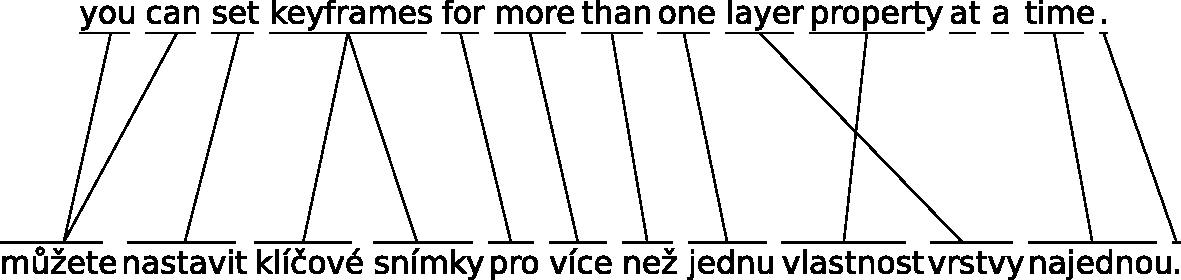
\includegraphics[width=\textwidth]{img/alignment/word_alignment_1_pdfa1a.pdf}
  \caption{\label{fig:word_alignment_1} Depiction of word alignment of the third sentence in WMT18 QE development data (English to German)"}
% You can set keyframes for more than one layer property at a time .
% Můžete nastavit klíčové snímky pro více než jednu vlastnost vrstvy najednou .
% 0-0 1-0 2-1 3-2 3-3 4-4 5-5 6-6 7-7 8-9 9-8 12-10 13-11
\end{figure}

Word alignment is the task of matching two groups of words in a bitext sentence if and only if they are each other's translations. An example\footnote{For the purposes of displaying word-alignment in the style of \cref{fig:word_alignment_1} and \cref{fig:word_alignment_2}, we wrote a small web-based tool SlowAlign. It is publicly available at \href{https://vilda.net/s/slowalign}{vilda.net/s/slowalign}. The source code is both hosted at \href{https://github.com/zouharvi/SlowAlign}{github.com/zouharvi/SlowAlign} and attached to this thesis.} of word alignment between an English sentence and translated German sentence can be seen in \autoref{fig:word_alignment_1}. Word alignment usually follows after sentence alignment.



\begin{figure}[ht]
  \centering
    \begin{tabular}{|c|c|c|c|c|c|c|}
        \hline
        & \rotatebox{90}{Klicken}
        & \rotatebox{90}{Sie}
        & \rotatebox{90}{mit}
        & \rotatebox{90}{der}
        & \rotatebox{90}{Maustaste\ }
        & \rotatebox{90}{.} \\
        \hline
        Click & \cellcolor{black} & \cellcolor{black} & \cellcolor{black} & & & \\ \hline
        the & & & & \cellcolor{black} & & \\ \hline
        mouse & & & & & \cellcolor{black} & \\ \hline
        button & & & & & \cellcolor{black} & \\ \hline
        . & & & & & & \cellcolor{black} \\ \hline
    \end{tabular}
  \caption{\label{tab:word_alignment_2} Bitext matrix of English to German word alignment}
\end{figure}

Sometimes the word alignment is depicted as in \cref{tab:word_alignment_2}, which is known as a bitext matrix. There is a point on $A_{i,j}$ if and only if the $i-$th source word is aligned to the $j-$th target word. Diagonal bitext alignment would correspond to a bitext matrix with points on its diagonal (a geometrical diagonal for non-square matrices). Sometimes it is impossible to do word alignment. Example of this are idiomatic phrases, whose translations can be idiomatic phrases in the target language and then there is no explicit mapping between individual words. We show such an example of only a partial matching in \cref{fig:word_alignment_2}. In this case using phrase-level alignment may be more suitable, as explored in \cite{bojar-prokopova:phrasal}. However, for most cases, we are able to construct meaningful word-level alignment.

\begin{figure}[ht]
  \centering
  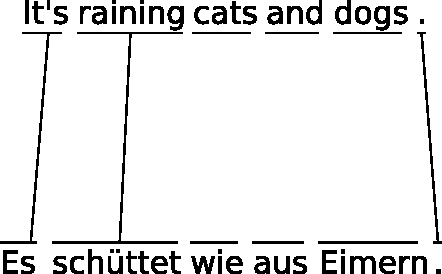
\includegraphics[width=0.36\textwidth]{img/alignment/word_alignment_2_pdfa1a.pdf}
  \caption{\label{fig:word_alignment_2} A partial alignment of an English idiom and its corresponding German translation.}
% It's raining cats and dogs .
% Es schüttet wie aus Eimern .
% 0-0 1-1 5-5
\end{figure}

For a long time, increasingly complex IBM Alignment Models 1 to 6 dominated the area of word-level alignment.\footnotehref{http://www.statmt.org/survey/Topic/IBMModels}{statmt.org/survey/Topic/IBMModels}  These models are a coproduct of statistical machine translation models. Summary of the development of IBM word alignment models can be found in the second chapter of \cite{cuvrin_alignemnt:2006}.

% There are two approaches to statistical word alignment. 
% Models 2 and 3 fix certain pitfalls of model 1. These improvements are penalization of translated words that are out of position and modelling probability of one word being translated into $n$ others. Model 3 implements a better solution to the fertility problem (modelling probability of an insertion). Model 4 introduced taking previously aligned words into account, while model 5 further refines this concept by penalizing the placement of two words in the same position. All of these five models were described in \cite{brown_ibm_1_2_3_4_5:1993}.  Model 6, the last model, stands out by combining model 4 with an alignment model based on Hidden Markov Models by \cite{vogel_hmm:1996}. 

Similarly to sentence alignment, research in the area of neural networks allowed for state-of-the-art results. An example of this can be found in \cite{legrand:2016}, where the authors use the dot product of windows from two convolutional layers (source and target) as the alignment score. As far as we know, none of the neural models has been made into a deployable word alignment tool. There are however hints of progress, as word alignment can be extracted from neural attention based machine translation systems, shown in Nizza\footnotehref{https://github.com/fstahlberg/nizza}{github.com/fstahlberg/nizza} and Neural Machine Translation.\footnotehref{https://github.com/tilde-nlp/neural-machine-translation-tools}{github.com/tilde-nlp/neural-machine-translation-tools}

The task of word alignment is formalized in \cite{mihalcea_evaluation:2003} together with four standard metrics: precision, recall, F-measure and quality of word alignment.

\pagebreak
\subsubsection{GIZA, GIZA++, MGIZA++, PGIZA++}
The GIZA word alignment collection is a standard used for this task. The first version, GIZA, was part of the EGYPT SMT toolkit and was later extended to GIZA++ and later became part of the Moses SMT toolkit.\footnotehref{http://www.statmt.org/moses/}{statmt.org/moses/}  It incorporates IBM Model 4, IBM Model 5 and Hidden Markov Models. The support for multithreading and clusters was later added, resulting in MGIZA++\footnotehref{https://github.com/moses-smt/mgiza}{github.com/moses-smt/mgiza} and PGIZA++\footnotehref{http://www.cs.cmu.edu/~qing/giza/}{www.cs.cmu.edu/\~qing/giza/}, respectively.

% It was presented in \cite{gizapp:2003}

In addition to word alignment, all of the ++ versions can perform some rudimentary form of sentence alignment.

\subsubsection{Fast\_align}
Fast align \citep{fastalign:2013} is a word aligner based on IBM Alignment Model 2, with improvements on this model's over-parametrization issues. It outperforms the commonly used IBM Alignment Model 4, is easy to build and use and has low resource requirements (both memory and computational time). It is often used as a baseline solution.

\subsubsection{Eflomal}
Eflomal\footnotehref{https://github.com/robertostling/eflomal}{github.com/robertostling/eflomal} is an improved version of Efmaral presented in \cite{ostling_efmaral:2016} together with comparison to the other two-word alignment systems. It is based on Bayesian alignment models with Markov Chain Monte Carlo inference. It is currently the state-of-the-art in word alignment.

\section{Machine translation}

The task of machine translation is to translate text from one language to another. In this context, it is strictly automatic and should not be confused with machine-aided human translation. This is an extensive topic and beyond the scope of this thesis. We thus provide only a very brief overview of the evolution and main approaches.

\subsection{Rule based (RBMT)}

First attempts for machine translation were made with rule-based systems, with either direct, syntactic or semantic transfer, which corresponds to steps described by the Vauquois triangle.\footnotehref{http://mttalks.ufal.ms.mff.cuni.cz/index.php?title=Intro\#Types\_of\_MT\_systems}{mttalks.ufal.ms.mff.cuni.cz/index.php?title=Intro\#Types\_of\_MT\_systems} Models based on the manipulation of morphological, syntactic and semantic structures are known as transfer based. They require linguistic knowledge of both source and target languages to be produced. We list examples of RBMT systems with short descriptions. Most of them became obsolete with the advent of statistical machine translation systems.

\begin{itemize}
    \item Ruslan - Created for Czech-Russian translation \citep{ruslan}.
    \item APAČ - Created for Czech-English translation \citep{apac}.
    \item METEO - Used for 20 years for English-French Canada weather reports translation \citep{meteo}.
    \item SYSTRAN - Developed by one of the oldest companies providing MT. It supports many language pairs and transitioned to SMT and NMT later \citep{systran}.
\end{itemize}

\subsection{Statistical (SMT)}
\label{subsec:smt}

Statistical machine translation models rely on a great amount of parallel data. They are usually modelled with two components: translation model and language model. This is shown in \autoref{eq:language_bayes} which shows the common application of the Bayes theorem for best translation $t$ given a source sentence $s$. The model is split into the translation model $p(s|t)$, evaluating translation relevance, and language model $p(t)$, which describes how well the proposed target sentence fits the language. The motivation is that monolingual data, used by the language model, are much easier to obtain than bilingual ones.

\begin{equation}
    \text{argmax}_t\ p(t|s) = \text{argmax}_t\ \frac{p(t)\cdot p(s|t)}{p(s)} = \text{argmax}_t\ p(s|t)\cdot p(t)
    \label{eq:language_bayes}
\end{equation}

The language model is usually modelled with n-grams. Its use made the translations more fluent as opposed to previous approaches.

SMT was first word-based, meaning words were manipulated and strung together to form a sentence. An example of this are the IBM models \citep{brown_ibm_1_2_3_4_5:1993}. More modern systems were phrase-based (documented in \citep{koehn2003statistical}), meaning whole sequences of words were manipulated and composed to form a sentence. This approach was widely adopted in the industry. We list examples of MT systems which are or were SMT based.

\begin{itemize}
    \item Google Translate - Is one of the most known publicly available MT system.\footnotehref{https://www.blog.google/products/translate/ten-years-of-google-translate/}{blog.google/products/translate/ten-years-of-google-translate/} It started transitioning to NMT in 2016.\footnotehref{https://www.blog.google/products/translate/found-translation-more-accurate-fluent-sentences-google-translate/}{blog.google/products/translate/found-translation-more-accurate-fluent-sentences-google-translate/}
    \item Bing Translator - Developed by Microsoft and is another widely used publicly available MT. It started transitioning to NMT in 2016.\footnotehref{https://www.microsoft.com/en-us/translator/business/machine-translation/}{microsoft.com/en-us/translator/business/machine-translation/}
    \item SYSTRAN - Was SMT, but partially transitioned to NMT in 2016.\footnotehref{http://kv-emptypages.blogspot.com/2016/12/systrans-continuing-nmt-evolution.html}{kv-emptypages.blogspot.com/2016/12/systrans-continuing-nmt-evolution.html}
\end{itemize}

\subsection{Neural (NMT)}

In the past decade, NMT systems became the state of the art and thus widely used. There are two main cornerstones of NMT: encoder-decoder and (self-)~attention. They both rely on recent advances in representation learning.

\subsubsection{Embedding}
One possibility to represent words in memory is using one hot encoding. Given a dictionary $D$, the $i$-th word of the dictionary would be represented by a vector of size $|D|$ of zeros except for one $1$ in the $i$-th place. This is far from the optimal approach, and there are many associated issues, such as data sparsity. In this encoding, each word form would be equally distant from each other. So the difference between the embeddings of \texttt{birds} and \texttt{bird} would be the same as between the embeddings of \texttt{birds} and \texttt{refrigerated}.

An alternative to this is to make a neural network learn a word representation. In this context, the representation is named \textit{word embedding}. Word2Vec \citep{word2vec} are types of networks, which can create such word embeddings out of monolingual data in an unsupervised way.
The authors propose two architectures. The first one is Continuous Bag-Of-Words, which tries to predict the current word based on the context, and the other is Skip-Gram, which tries to predict the context based on the current word. 
% \footnote{The tokens in the data are actually in sequence and not just a set. So the context of the word is the supervision.}

Word embeddings are able to capture relationships between embedded words. So word embeddings for \texttt{birds} and \texttt{bird} would be closer together than the word embeddings for \texttt{birds} and \texttt{refrigerated}.

Another improvement was the introduction of subword units and relevant training algorithms, such as Byte Pair Encoding \citep{subwords_bpe}. Subword units are used to deal with unseen and rare words. If a word is too rare, it will not get its own word embedding but will be split into multiple subword units. This is intuitive, as humans are able to understand new words by analyzing their morphemes.

\subsubsection{Encoder-Decoder}
The encoder-decoder architecture is the standard approach for sequence to sequence tasks. In this case, it is a sequence of word embeddings, which is passed to multi-level bidirectional RNN, composed of either Long Short Term Memory (LSTM) or Gated Recurrent Unit (GRU). The result is called the hidden state, and it is a fixed-size vector, which is passed between the cells. The hidden state represents the whole input sentence. To get the translated output, the hidden state is unrolled with the same mechanism, but this time the probabilities of all possible output subword units are produced. A search algorithm, possibly a greedy one, selects one of them and the decoder moves to the next step.


% word embeddings are outputted. They are then mapped to subword units (with target embedding) and form the output sentence. 



The actual recurrent neural networks used for machine translation are made more complex, such as with the use of multiple layers of encoders.

\subsubsection{Attention}

One of the deficiencies of the purely encoder-decoder approach is that both of the RNN components only have direct access to the immediately preceding word. This is a problem in case the translation of the current word is dependent on a word, which was either encountered (source) or generated (target) several steps back. Such distant word is embedded in the hidden state (fixed size vector), but it may be too difficult to extract its features.

A novel approach was taken by \cite{bahdanau2014neural}. They proposed a system by which a current (to be produced) word can reference the words the translation is dependent on. Such referencing is called the attention mechanism and there are two types usually distinguished: global attention and local attention. This mechanism is employed only in the decoder part and the attention mechanism adds a context vector to the word translation computation.

Global attention computes the context from all of the source words using a hidden alignment vector, which supplies weights for each word. Local attention focuses on a window of a fixed size around the aligned source word.

Popular MT models such as Transformer \citep{attention_all_you_need} or BERT \citep{bert} make use of attention mechanisms and add other improvements, such as multi-head self-attention. As is apparent from the transition in the industry standard in the listing in \cref{subsec:smt}, NMT together with attention mechanisms outperforms SMT and it is now the state of the art and widely used.

\subsection{Evaluation}

Automatic machine translation evaluation assigns scores to the produced machine translations, given also the source text and reference translation. The goal is to find such a metric, that would correlate the most with human annotations. This is not an easy task to automate, as the machine translation can be vastly different from the reference translation, but still be correct. Alternatively, it can be very close to the reference translation, but be very ungrammatical or can distort the meaning seriously.

Many other metrics have been proposed and this area of research is still active. The metrics shared task is part of WMT \citep{wmt19_metrics}.

\subsubsection{BLEU}
Bilingual Evaluation Understudy \citep{bleu} is the most common metric for evaluation of MT systems. It is based on searching for n-grams in the translated sentence, which are also in the reference translation. The geometric mean of unigram, bigram, trigram and quadrigram precision is calculated and the score computed as in the formula in \cref{fig:bleu}. 

The first part of the product is called the \textit{brevity penalty}. It is there to make sure that the MT system does not game the metric by outputting for example only one quadrigram, which it is very sure about. In this case all of the precisions would be close to $1$, but human annotators would not consider this to be a good translation.

\begin{equation}
    \text{BLEU} = exp\big(\min(1, 1-\frac{\text{output length}}{\text{reference length}})\big) \cdot \big(\prod_{i=1}^4 \text{prec}_i\big)^\frac{1}{4}  
    \label{fig:bleu}
\end{equation}

\subsubsection{METEOR}
Metric for Evaluation of Translation with Explicit ORdering aims to fix some disadvantages of BLEU. In contrast to BLEU, it considers only unigrams and not bigrams, trigrams, nor quadrigrams. It uses stemming and synonyms and tries to create mappings between the translated and reference sentence. It has been shown \citep{meteor} that it correlates better with the human judgement than BLEU.

\subsubsection{Round trip translation}

Also called backward translation, round trip translation is an idea of evaluating an MT system without reference. It is based on translating the source sentence to a foreign language and then back and measuring BLEU score between source and backward translated text. In \citep{rtt_what_is_it_good_for} it was demonstrated, that RTT does not correlate with the quality of MT systems in any statistically meaningful way.

\section{Quality estimation}
As opposed to machine translation evaluation, which uses source text and target and reference translations to evaluate the output, the objective of quality estimation (also known as confidence estimation) is to predict the translation quality without reference translations.

Machine translation quality estimation aims to provide hints as to whether a produced machine translation is good or bad. Quality estimation shared task was part of WMT since 2012\footnotehref{http://www.statmt.org/wmt12/quality-estimation-task.html}{statmt.org/wmt12/quality-estimation-task.html} and was forked from automatic machine translation evaluation shared task, which was part of WMT since 2008\footnotehref{http://www.statmt.org/wmt08/shared-evaluation-task.html}{statmt.org/wmt08/shared-evaluation-task.html} and in 2012 renamed to metrics task. The results of the latest findings of the WMT quality estimation shared task 2019 are discussed in \citep{wmt_qe:2019}.

The input of metrics task, as defined by WMT, is the translation together with human reference translations. It is performed usually on sentence-level and system-level. In contrast, the input for quality estimation system is the source text and the translated text. Quality estimation is then performed on word-level, phrase-level and sentence-level.

For document-level quality estimation, the document is either to be assigned a score, or the system should report spans, which contain translation errors. The quality of sentence-level quality estimation is measured in HTER (edit-distance metrics).


The output of word-level quality estimation is usually a list of probabilities for each token in the target sentence. In WMT, the format is only binary values for each token. For word-level quality estimation models, to encapsulate missing words, tokens for gap were added. Thus each space adjoining a target token can also be classified as \texttt{OK} or \texttt{BAD}, denoting a missing word in the latter case. For $N$ target tokens, $2\cdot N + 1$ binary values should be generated. This is illustrated in \autoref{fig:word_level_gaps}.

\begin{figure}[ht]
  \centering
  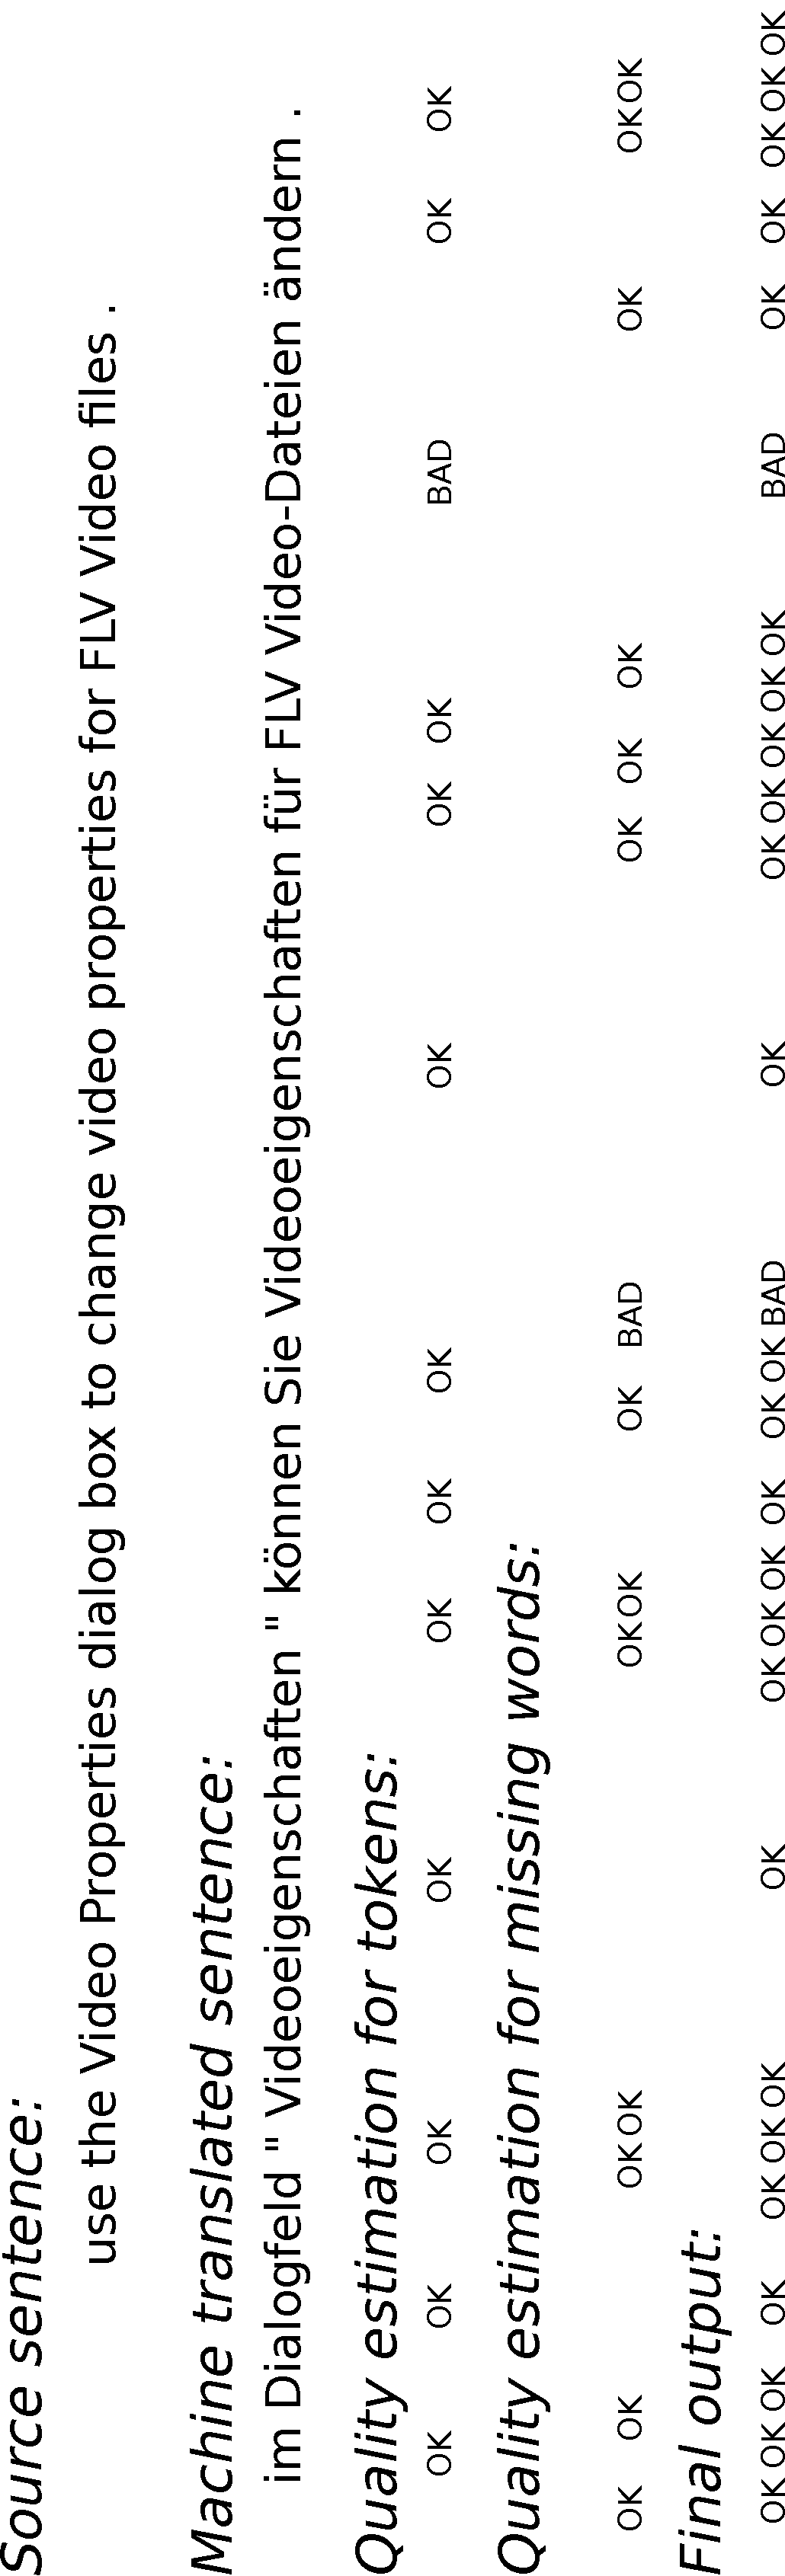
\includegraphics[height=\textwidth, angle=-90]{img/quality_estimation/format_pdfa1a.pdf}
  \caption{\label{fig:word_level_gaps} Quality estimation tags for tokens and gaps on German sentence translated from English (from WMT19 quality estimation shared task)}
\end{figure}

\pagebreak
\subsection{QE from machine translation models}
Some machine learning systems, especially classifiers, are able to report also the confidence in their output. To our knowledge, quality estimation from the machine translation models themselves is used only in combination with another QE system which use this self-reported confidence as one of the features.

\subsection{QuEst++}
The main pipeline of QuEst++ by \cite{questplusplus} consists of feature extraction and machine learning prediction. This system first extracts features from the input data and then runs a machine learning algorithm for example with scipy's LarsCV (Cross-validated Lasso, using the LARS algorithm) or Conditional Random Fields suite by \cite{CRFSuite}.

A large part of their work is devoted to feature exploration and fine-tuning. There are four groups of features for word-level quality estimation:

\begin{itemize}
    \item word alignment
    \item POS of source and target words
    \item n-gram frequencies in source and target texts
    \item syntactic, semantic and pseudo-reference binary flags
\end{itemize}

They are an extension of features for word-level quality estimation used by WMT12-13-14-17-18 for the baseline model.\footnotehref{https://www.quest.dcs.shef.ac.uk/quest\_files/features\_blackbox\_baseline\_17}{quest.dcs.shef.ac.uk/quest\_files/features\_blackbox\_baseline\_17} For sentence-level, the features are focused on the relations of tokens in the source and target sentences, e.g. the ratio of such tokens and distribution of parts of speech. Document features incorporate aggregation of sentence-level features as well as features on the discourse level by \cite{scarton_reading:2016}.

Since the system was not designed to provide online results, the consequence is, that especially the feature extraction part is not optimized and is quite slow. It can handle only ten sentences at a time, so larger inputs have to be split into multiple batches. At the time of deployment there were two bugs, for which we opened pull requests.\footnote{\href{https://github.com/ghpaetzold/questplusplus/pull/45}{github.com/ghpaetzold/questplusplus/pull/45} and \\ \ttab[0.5] \href{https://github.com/ghpaetzold/questplusplus/pull/46}{github.com/ghpaetzold/questplusplus/pull/46}}


\subsection{DeepQuest}
DeepQuest \citep{deepquest} takes a neural approach to quality estimation and is capable of performing on any language pair. The toolkit offers two architectures.

\begin{figure}[H]
  \centering
  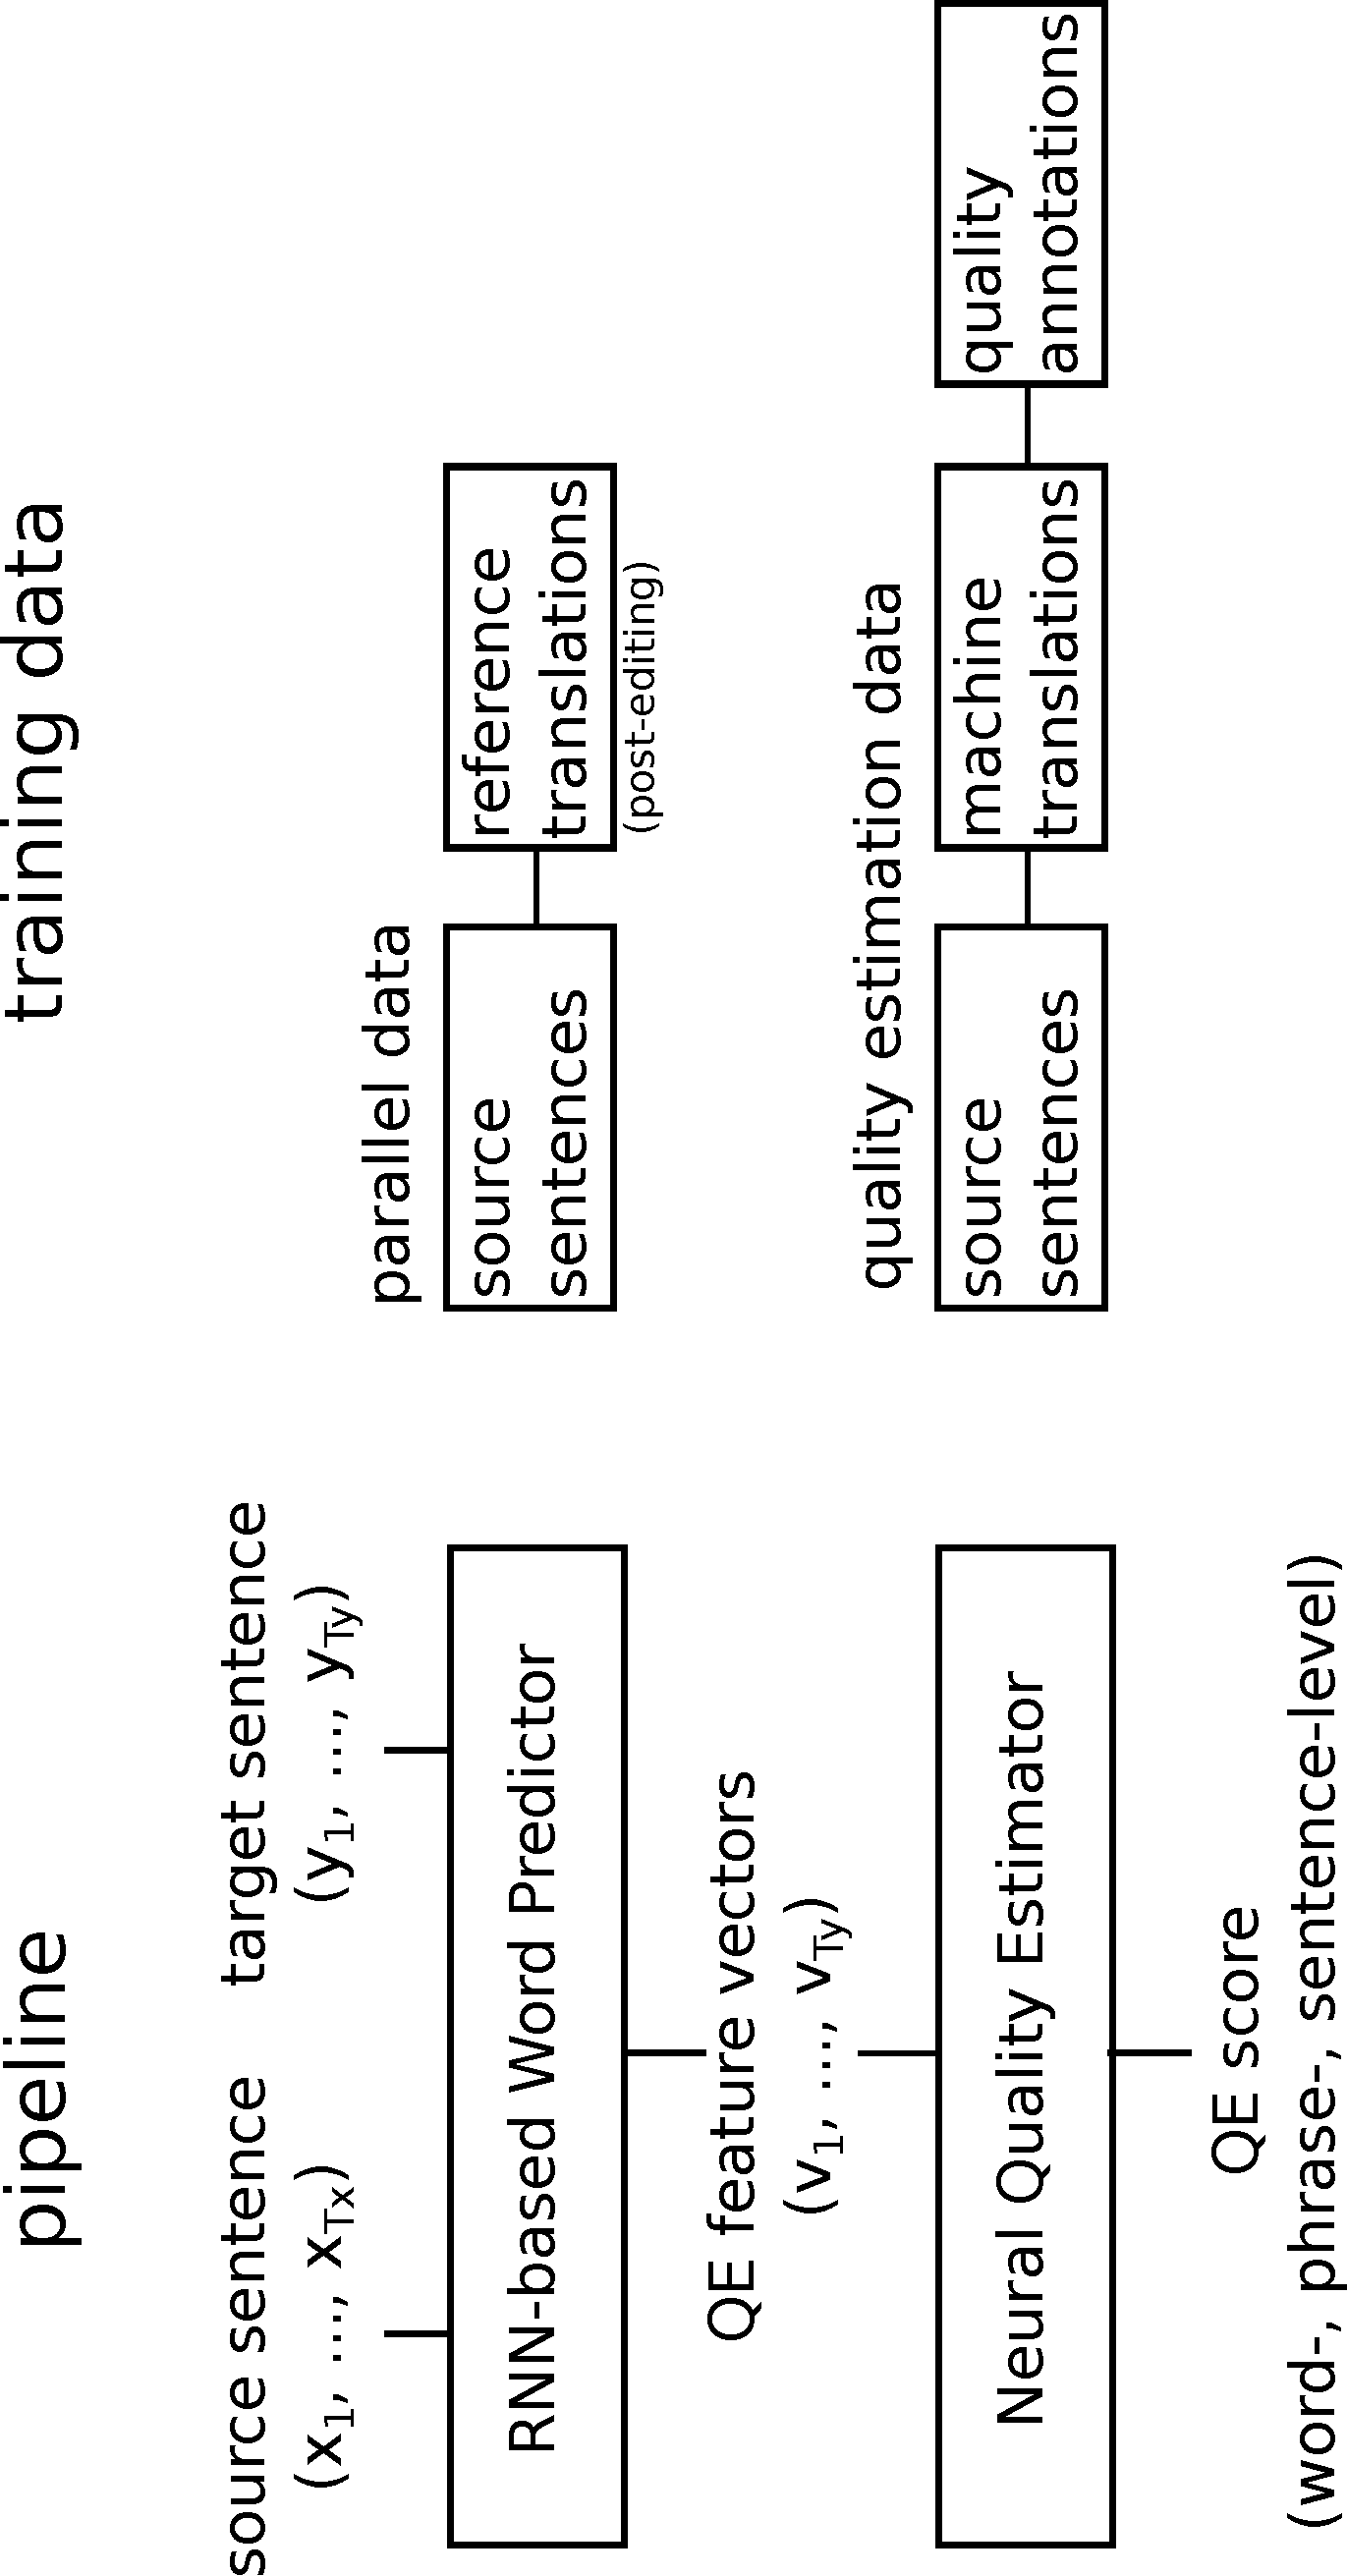
\includegraphics[height=0.9\textwidth, angle=-90]{img/quality_estimation/postech_architecture_pdfa1a.pdf}
  \caption{\label{fig:postech_architecture} Predictor-Estimator QE model pipeline and type of training data, adapted from Fig. 1 from \citep{Kim-Postech:2017}}
\end{figure}

Predictor-Estimator architecture \citep{Kim-Postech:2017} consists of two stages of training. In the first one, a predictor (encoder-decoder RNN) is trained on parallel data to predict words based on their context representations. Feature vectors from this network are then passed to the estimator, which is trained on quality estimation data. This delegates the issue of feature engineering onto machine learning itself. The architecture is illustrated in \autoref{fig:postech_architecture}.

The other architecture implemented by DeepQuest is biRNN. A sequence is passed into RNN both in the original ordering as well as in reverse. The results are then concatenated and propagate further into the rest of the network. The network can then make use of not only the preceding item in the sequence but also the subsequent one.

Models of both architectures can be executed on document-level, sentence-level, phrase-level and word-level.

\cite{deepquest} reported better results in most experiments on WMT17 with the Predictor-Estimator than the baseline (QuEst++). Performance of the biRNN architecture is still better than the baseline and does not significantly lack behind the Predictor-Estimator. They also stress the difference of performance of implemented systems on SMT and NMT data, with the later resulting in worse results, presumably because the error is less predictable in the latter case.

Despite the better results, we found the implementation difficult to work with because of several bugs. Even though some of the bugs we reported were fixed, the latency of this tool was still too high for online purposes.

\subsection{OpenKiwi} \label{subsec:openkiwi}

OpenKiwi \citep{openkiwi} implements three quality estimation models: QUality Estimation from ScraTCH \citep{kreutzer-quetch:2015}, NeUral Quality Estimation \citep{martins-unbabel:2016} used for WMT19\footnotehref{http://www.statmt.org/wmt19/qe-task.html}{statmt.org/wmt19/qe-task.html} baseline and Predictor-Estimator \citep{Kim-Postech:2017}. In addition OpenKiwi implements stacked ensemble as proposed in \cite{martins-ms:2017}.

QUETCH is a linear combination of baseline features and custom neural network. The architecture of the later is shown in \autoref{fig:quetch_architecture}. For each target token $t_i$ an aligned source token $s_{a(i)}$ is considered. Then windows of size three are concatenated: $(t_{i-1}, t_i, t_{i+1}, s_{a(i)-1}, s_{a(i)}, s_{a(i)+1)}$ and passed through a lookup-table (pretrained word2vec). The resulting vectors are then passed through a densely connected layer and finally through an output layer, which outputs \texttt{OK} or \texttt{BAD}.

\begin{figure}[ht]
  \centering
  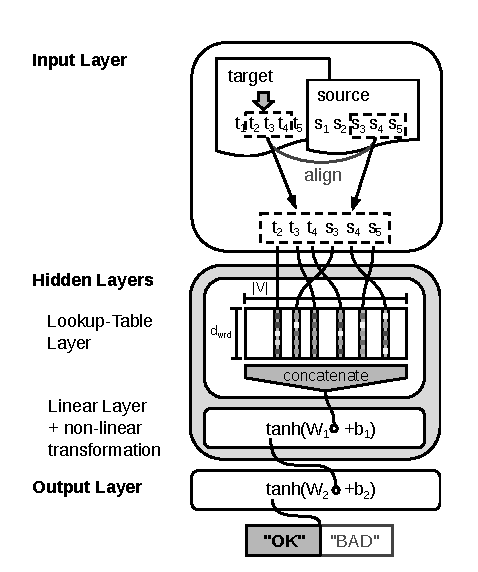
\includegraphics[width=0.6\textwidth, angle=0]{img/quality_estimation/quetch_architecture_pdfa1a.pdf}
  \caption{\label{fig:quetch_architecture} QUETCH model architecture, from Fig. 1 in \citep{kreutzer-quetch:2015}}
\end{figure}

NuQE is very similar to QUETCH in most respects. In addition, POS tags are concatenated and passed through a POS embedding table and finally, two layers bidirectional gated recurrent units are appended (with two extra dense layers in between).

We opted for the Predictor-Estimator architecture because even though it requires pretraining, it does not consume many resources compared to the stacked ensemble. Except for the ensemble, it also provides the best results as shown in \cite{openkiwi}. OpenKiwi, in general, proved to be faster, more robust and easier to use\footnote{OpenKiwi is distributed via pip \href{https://pypi.org/project/openkiwi/}{pypi.org/project/openkiwi/} as a Python module.} than DeepQuest. Because of this, the experiment was conducted with this quality estimation backend.

\subsection{Evaluation}

Since the output of sentence-level and phrase-level quality estimation is usually HTER, there are several metrics for quality estimation systems. They are measured over the whole dataset.

\begin{itemize}
    \item Root Mean Squared Error
    \item Mean Average Error
    \item Pearson's correlation
    \item Spearman's rank correlation
\end{itemize}

For word-level quality estimation, the output is a sequence of probabilities, which can be, for a given threshold, transformed into a sequence of two classes \texttt{OK} and \texttt{BAD}. Since the distribution of \texttt{OK} and \texttt{BAD} for most of the sentences is unbalanced, accuracy could be cheated by predicting always \texttt{OK}. To balance precision and recall, F measure with respect to \texttt{OK} and \texttt{BAD} is used. To incorporate both, $F_{MULTI} = F_{OK}\cdot F_{BAD}$ is usually used as a metrics for WMT quality estimation task.

\section{Source complexity}

The task of estimating source complexity is not rigidly defined and has not been thoroughly explored. In the context of machine translation, we can think of it as finding patterns in a sentence which are hard to translate by MT systems. For our purposes, it is beneficial to know which parts of the source sentence are challenging to translate, so that users speaking only the source language can reformulate that specific segment.

\subsubsection{Lexical choice}

One of the most straightforward ideas would be to look at individual words in the source sentence and describe the probability of them being translated correctly. This can be done, for example, by searching for that word in the data the specific MT system used for training. Subword units can help with unseen words, but we can still hypothesize, that if a word has never been seen by an MT system, it will be difficult to translate.

Another approach to recognize problematic source words would be using word alignment and word-level quality estimation. A QE system gives a score to every translated word. These values can be mapped back to the source sentence by word alignment. This approach was chosen for \ptakopet{} because it could be done with already existing tools. The implementation is discussed in \cref{subsubsec:impl:source_complexity}.

\pagebreak
\subsubsection{Syntactic structures}

For most MT systems it is not a single unknown word which worsens the translation quality but syntactic structures. This has been described extensively in \cite{choshen_challenge_sets}. Their claim is that long distance dependencies are still a massive problem for translation quality.

The work of \cite{niehues_confidence} focuses not only on target tokens QE but also on confidence annotation of source tokens. Their methods are based on complex similarity measures between the given source sentence and training data.